%!TEX root = ../rapport.tex

\chapter{Analyse de l'application générale}
Le but de ce chapitre est de décrire l'analyse qui a été faite au début du projet afin de faciliter le déroulement des étapes suivantes comme la conception, l'implémentation et les tests du système.

\medskip

Cette partie décrit l'analyse du projet en général. L'analyse plus spécifique de la partie \emph{client} et \emph{serveur} se fait, respectivement, dans la section \ref{sec:analyse_client} et \ref{sec:analyse_serveur}.

\section{Base de données} % (fold)
\label{sec:base_de_donn_es}
La base de données pour le projet existe déjà. Néanmoins, il n'est pas impossible qu'il y aura des changements à effectuer pour répondre correctement aux besoins de l'application. Cette base de données résulte de modifications et d'ajouts sur celle utilisée pour le projet Watt-ICT. En effet, l'\gls{eiafr} a repensé certains points du modèle de données afin de partir avec une meilleure base.

\medskip

La figure \ref{gra:bddv2} est le résultat du travail sur la base de données avant le projet.

\medskip

En analysant la base de données, nous pouvons nous apercevoir des faits suivants : 

\medskip

\begin{itemize}
    \item Un utilisateur peut avoir une, plusieurs ou aucune maisons
    \item Les maisons peuvent être reliées à plusieurs utilisateurs
    \item Une zone ne peut être reliée qu'à une seule maison
    \item Une zone peut être reliée à plusieurs capteurs
    \item Un capteur ne peut être relié qu'à une seule zone
    \item Les capteurs sont reliés à des données capturées et il existe une table qui permet de récuperer les dernières données du capteur
    \item Chaque donnée est reliée à un autre type avec lequel on peut récupérer le nom, l'unité, etc...
    \item On peut déjà voir qu'il y aura des champs à ajouter concernant l'image du plan
    \item Il faudra également ajouter des positions pour le plan, une largeur, une hauteur
    \item Même constatation pour les zones puisqu'il faudra savoir où elles doivent être placées, la largeur et la hauteur
\end{itemize}


\begin{figure}[H]
    	\centering
    	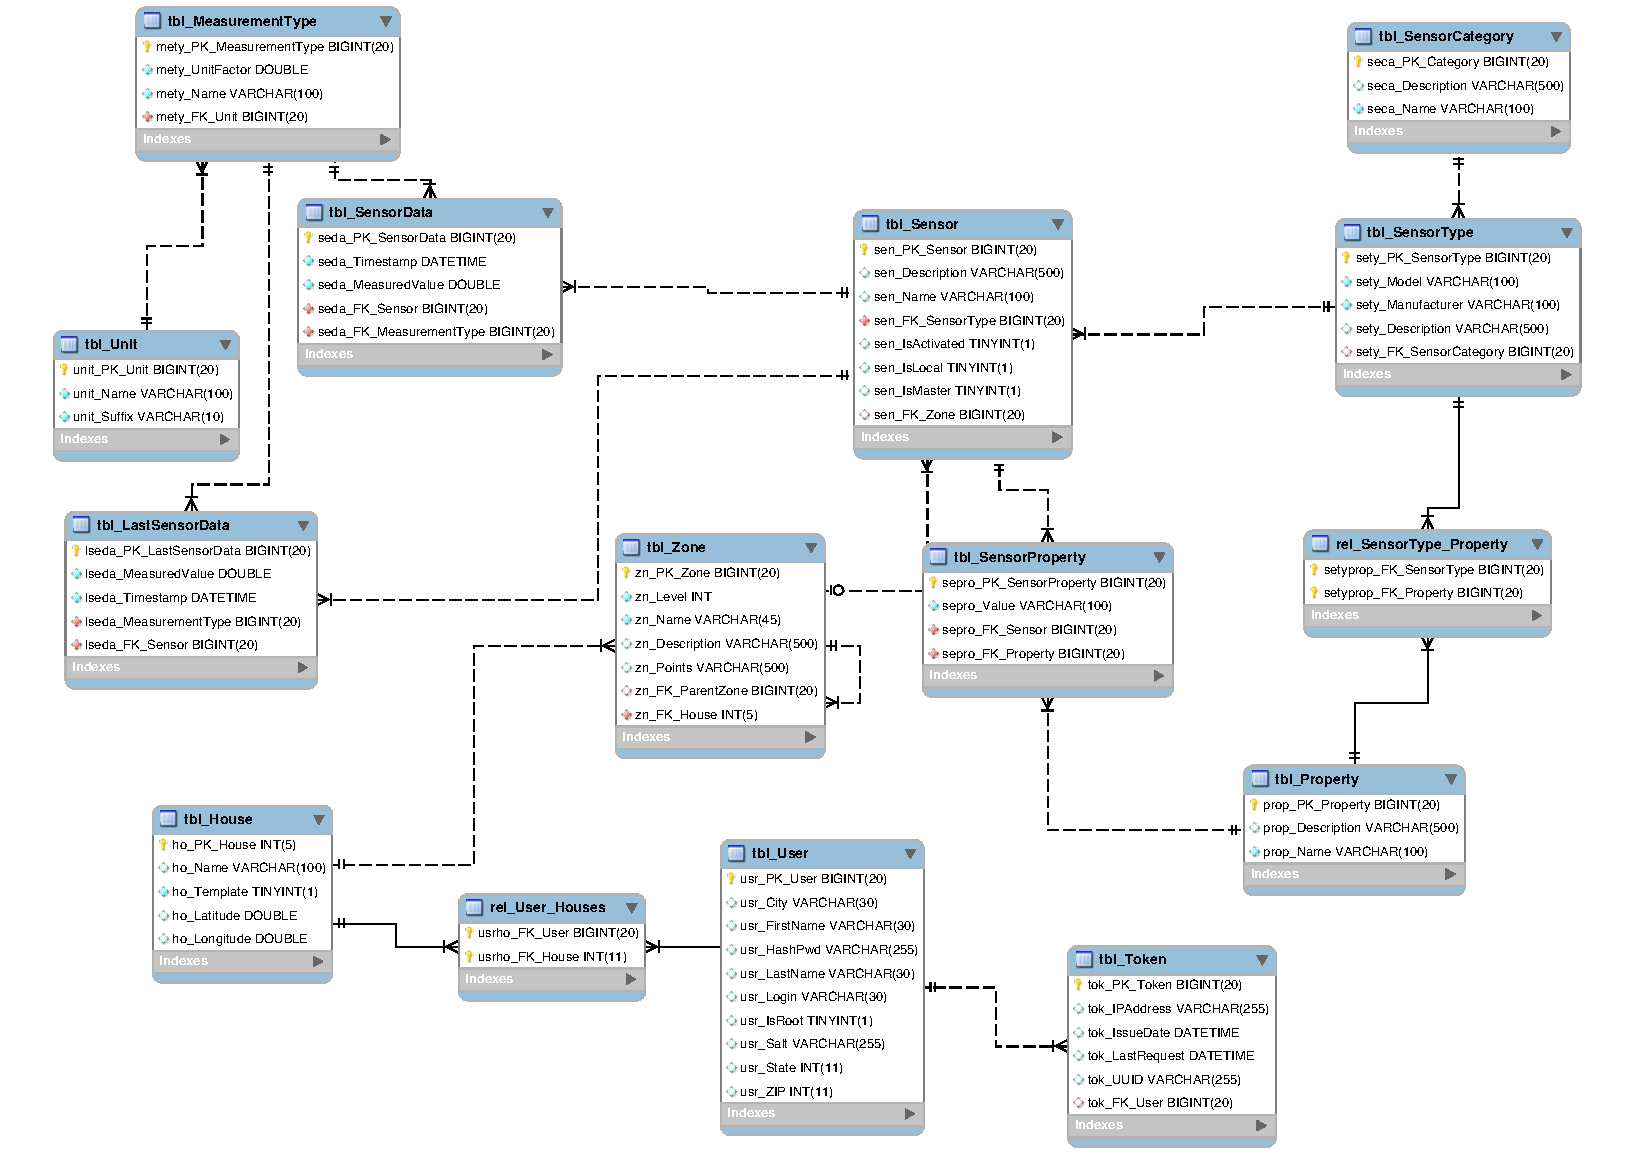
\includegraphics[width=\textwidth]{00_media/03_bddV2.pdf}
    	\caption{Base de données avant le projet}
    	\label{gra:bddv2}
\end{figure}
% section base_de_donn_es (end)


\section{Prise en main de Watt-ICT} % (fold)
\label{sub:etat_actuel_du_syst_me}
Il existe actuellement une plateforme qui permet de gérer des capteurs dans différentes maisons. Cette application permet en effet d'ajouter des maisons pour ensuite les lister avec leurs capteurs associés. De plus, elle permet d'avoir des informations sur la fréquence, la puissance, etc.. Ce projet a donc un but écologique puisqu'il permet de récupérer des données intéressantes en vue de faire de l'économie d'énergie.

\medskip

Malheureusement, cette plateforme comporte certains bugs, n'est pas des plus conviviales à utiliser et ne présente aucune documentation. De plus, les personnes travaillant à l'EIA-FR trouvent que la base de données n'est pas très bien pensée et c'est pour cette raison qu'ils l'ont redesignée pour des projets à l'école.

\medskip

Il faudra donc reprendre les meilleures parties, les adapter et implémenter les éléments indispensables au bon fonctionnement du projet.

\medskip

Cette section décrit les étapes qui ont été nécessaires afin de pouvoir démarrer la plateforme \emph{Watt-ICT}. Les deux étapes principales sont la mise en place de la base de données et la configuration d'\emph{\gls{eclipse}}
\subsection{Mise en place de la base de données} % (fold)
\label{sub:mise_en_place_de_la_base_de_donn_es}
Le plateforme nécessite la mise en place d'une base de données pour pouvoir récupérer les informations. Pour se faire, j'ai utilisé \emph{\gls{mamp}} dans sa version 2.0.5.

\medskip

Pour mettre en place la base, j'ai utilisé le fichier \emph{\gls{sql}} disponible sur la Forge à l'adresse \url{https://forge.tic.eia-fr.ch/attachments/download/2910/dump.sql}. J'ai simplement utilisé la fonction qui permet d'importer un fichier contenant du code \emph{\gls{sql}}.

\medskip

Voici les informations nécessaires pour la suite:

\medskip

\begin{itemize}
 	\item Hôte : {\bf localhost}
 	\item Port : {\bf 8889}
 	\item Utilisateur : {\bf root}
 	\item Mot de passe : {\bf root}
 	\item Nom de la base : {\bf green-app}
 \end{itemize} 
% subsection mise_en_place_de_la_base_de_donn_es (end)

\subsection{Configuration d'Eclipse} % (fold)
\label{sub:eclipse}

% subsection eclipse (end)
Afin de lancer le programme Watt-ICT, il a été nécessaire d'effectuer plusieurs opérations. Pour commencer, j'ai utilisé \emph{\gls{eclipse}} dans sa version 3.7.2. Voici la marche à suivre qui a été suivie afin de pouvoir accéder à la plateforme.

\medskip

Pour commencer, afin de pouvoir importer un projet \emph{\gls{maven}}, il faut,  dans \emph{\gls{eclipse}}, installer les plugins suivants à l'aide du menu \emph{Help} en cliquant sur \emph{Install New Software} :

\medskip

\begin{itemize}
    \item \emph{Subversive Site} disponible grâce à l'adresse \cite{online:eclipse:subversive}
    \item \emph{Maven Integration for Subclipse} disponible grâce à l'adresse \cite{online:eclipse:mavensubclipse}
    \item \emph{Maven SCM Handler for Subversive} disponible grâce à l'adresse \cite{online:eclipse:scm}
\end{itemize}

\medskip

Une fois ceci fait, il est possible de créer un nouveau projet \emph{\gls{maven}} en faisant un \emph{Checkout} comme le montre la figure \ref{gra:mavenProjectCheckout}.

\begin{figure}[H]
    	\centering
    	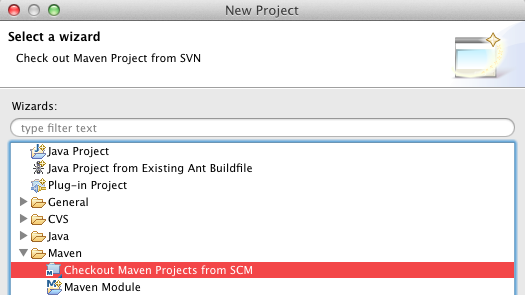
\includegraphics[width=300px]{00_media/02_mavenProjet.png}
    	\caption{Création d'un nouveau projet Maven}
    	\label{gra:mavenProjectCheckout}
\end{figure}

Il faut ensuite sélectionner le type d'url \emph{(svn)} et entrer son adresse qui est \url{https://forge.tic.eia-fr.ch/svn/eiafr/tic/acad/info/1112/igreencontrol/trunk}. On peut désormais directement cliquer sur \emph{Finish}.

\medskip

Lorsque ceci est fait, un nouveau projet apparaît. Il faut encore éditer le fichier de configuration pour accéder à la base de données qui a été mise en place précédemment. Ce fichier se nomme \emph{ga-service.conf} et le code \ref{lst:bddConfig} montre le contenu qui a été inséré.

\begin{lstlisting}[language={XML}, caption={Fichier de configuration BDD}, label={lst:bddConfig}]
# Database access parameters
db.url = jdbc:mysql://localhost:8889/green-app
db.user = root
db.password = root

# HTTP parameters
http.url = localhost/ga-service
http.port = 9998
\end{lstlisting}

Il est maintenant possible d'accéder à la plateforme via l'adresse \url{http://localhost:9998/ga-service/index.html}
% section etat_actuel_du_syst_me (end)
